\section{Assessing Reservoir Conditions}\label{sec:evaluation}

In this section I evaluate map-derived tilt-distance datasets generated in Section~\ref{sec:mapping} by comparison with model tilt-distance solutions from Section~\ref{sec:modeling}. The ultimate goal is to estimate an array of magma reservoir parameters---center position (map view), depth, radius (map view), aspect ratio, and pressure change---most consistent with the discordant flows at the surface. 

Among these five parameters of interest, reservoir center position must be assessed first because it alone dictates the tilt-distance dataset implied by a discordant set of features. This derived tilt-distance dataset can then be compared with an array of tilt-distance solutions derived from numerical models incorporating the other four parameters.

\subsection{Center Position}

Figure~\ref{fig:candidates} illustrates the array of candidates to be assessed as possible reservoir center locations. Section~\ref{sec:mapping} introduces the construction of a single tilt-distance data point from one discordant sample point relative to one center location. Repeating this calculation for all sample points relative to one center yields a full tilt-distance dataset corresponding to that center.\footnote{Figure~\ref{fig:tilt-example} illustrates instead repeating this calculation for a single sample point relative to all possible centers.} By repeating this construction, each center candidate can finally be evaluated on the basis of its associated tilt-distance dataset. In general, this means each dataset is reduced to a small set of numerical scores. This approach is outlined in Figure~\ref{fig:eval-model} and implemented in Appendix~\ref{app:code}.

\begin{figure}
    \begin{tikzpicture}[scale=.95]

  \usetikzlibrary{positioning}

\coordinate (ceval) at (0,0);
\coordinate (centersample) at (0,5);
\coordinate (samples) at (-3,10);
\coordinate (centers) at (3,10);

\node [rotate=270] at (7, 10) {Input (from GIS)};
\node [rotate=270] at (7, 5) {Intermediate list};
\node [rotate=270] at (7, 0) {Output (back to GIS)};

\draw[arrow,line width=1mm] (6, 10) -- (6, 0);

\node (samplestable) [draw, shape=rectangle, align=center] at (samples) {\begin{tabular}{c|c}
    sID & LAT, LON, \acs{az1}, \acs{az2}, \acs{sl2}\\
    \hline\\
    \hline\\
    \hline\\
    \hline\\
  \end{tabular}};

\node[above=0mm of samplestable] {\hltt{samples.csv}};

\node (centerstable) [draw, shape=rectangle, align=center] at (centers) {\begin{tabular}{c|c}
    cID & LAT, LON\\
    \hline\\
    \hline\\
    \hline\\
    \hline\\
    \hline\\
    \hline\\
  \end{tabular}};

\node[above=0mm of centerstable] {\hltt{centers.csv}};

\node (frontcentersample) [shape=rectangle, align=center, rounded corners=0.2cm] at (centersample) {\begin{tabular}{c|c|c}
  sID & LAT, LON, \acs{az1}, \acs{az2}, \acs{sl2} & \acs{dist}, \acs{bearing}, \acs{beta1}, \acs{beta2}, \acs{sl1}, \acs{tilt}\\
  \hline
  &\\
  &copy of & calculated\\
  &\hltt{samples.csv} & from one cID\\
  &\\
\end{tabular}};

\node[above=3mm of frontcentersample] {\hltt{centers\_calc}};

\foreach \x in {0.3,0.25,...,-0.05}
    \path (centersample) + (-\x, \x) node[draw, shape=rectangle, align=center, fill=white, rounded corners=0.2cm] {\begin{tabular}{c|c|c}
        sID & LAT, LON, \acs{az1}, \acs{az2}, \acs{sl2} & \acs{dist}, \acs{bearing}, \acs{beta1}, \acs{beta2}, \acs{sl1}, \acs{tilt}\\
        \hline
        &\\
        &copy of & calculated\\
        &\hltt{samples.csv} & from cID\\
        &\\
      \end{tabular}};

  \node (centersevaltable) [draw, shape=rectangle, align=center] at (ceval) {\begin{tabular}{c|c|c}
    cID & LAT, LON & SCORES\\
    \hline
    &\\
    &\\
    &copy of&each row calculated from\\
    &\hltt{centers.csv}&one item in \hltt{centers\_calc} \\
    &\\
    &\\
  \end{tabular}};

\node[above=0mm of centersevaltable] {\hltt{centers\_eval.csv}};

\end{tikzpicture}%
    \caption[Center evaluation workflow]{Schematic illustration of candidate center evaluation process. For each center (unique cID) in \hltt{centers.csv}, I make a copy of \hltt{samples.csv} and calculate variables for each sample (unique sID). This results in the ``intermediate list'' where each element corresponds to one cID. Then I evaluate each item in this list and write the resulting scores to one row of \hltt{centers\_eval.csv}.}%
    \label{fig:eval-model}
\end{figure}

Two broad questions inform the numerical scores assigned to each center based on its associated tilt-distance dataset:
\begin{enumerate}
    \item How well does the dataset capture the mapped discordant features?
    \item How well does the dataset capture a plausible modeled reservoir change event?
\end{enumerate}
Naturally, the best centers are the ones whose datasets can explain both the discordant features and a plausible reservoir change event. The following sections provide specific answers to these two questions. 

\subsubsection{Valid Fraction (Tiltable \& Offset)}\label{sec:valid-fraction}

Section~\ref{sec:tiltable} introduces the ``tiltable'' criterion for samples with respect to a particular inflation center location. In particular, tilt estimates can only be obtained for certain values of the ``direction-away-from-center'' (\acs{bearing}) variable. The directions \emph{toward} these impossible centers are illustrated as the blank gaps in the colorful rims of Figures~\ref{fig:tilt-example} and~\ref{fig:tilt-behavior} and described quantitatively in Section~\ref{sec:paleo-slope} (esp. Equation~\ref{eq:paleo-slope}).

However, even among the tiltable centers for a particular center,\footnote{Or, for this section, the tiltable \emph{samples} for a given \emph{center}.} it is also important to consider the reliability of the calculated tilt values. Notice in Figure~\ref{fig:fig:tilt-behavior} that the highest-magnitude tilt calculations are densely clustered along one side of the \acs{bearing} line. The steep color gradient in this region indicates that tilt is sensitive to small variation in azimuth measurements of modern attitude, flow orientation, or center position. This unpredictable behavior approaches the undefined solution where the flow feature is colinear with the center candidate ($\beta1=\ang{0}$ or $\beta1=\pm\ang{180}$): no amount of tilt about the imposed axis can change the azimuth of the flow, so no tilt can be inferred from discordance (also illustrated in Figure~\ref{fig:discordance-concept}).

To avoid error-prone results captured by this phenomenon, I introduce an ``offset'' boolean criterion to complement the tiltable criterion. This criterion is simply a minimum cutoff value of \acs{beta1} of \ang{7}, chosen to capture most of the unstable behavior for typical attitude data in this thesis. More precisely, an ``offset'' sample relative to a particular center candidate is one where the absolute value of \acs{beta1} is greater than \ang{7} and less than $\ang{180}-\ang{7}=\ang{173}$. The tiltable and offset criteria are illustrated in Figure~\ref{fig:tiltable-offset}.

\begin{figure}
    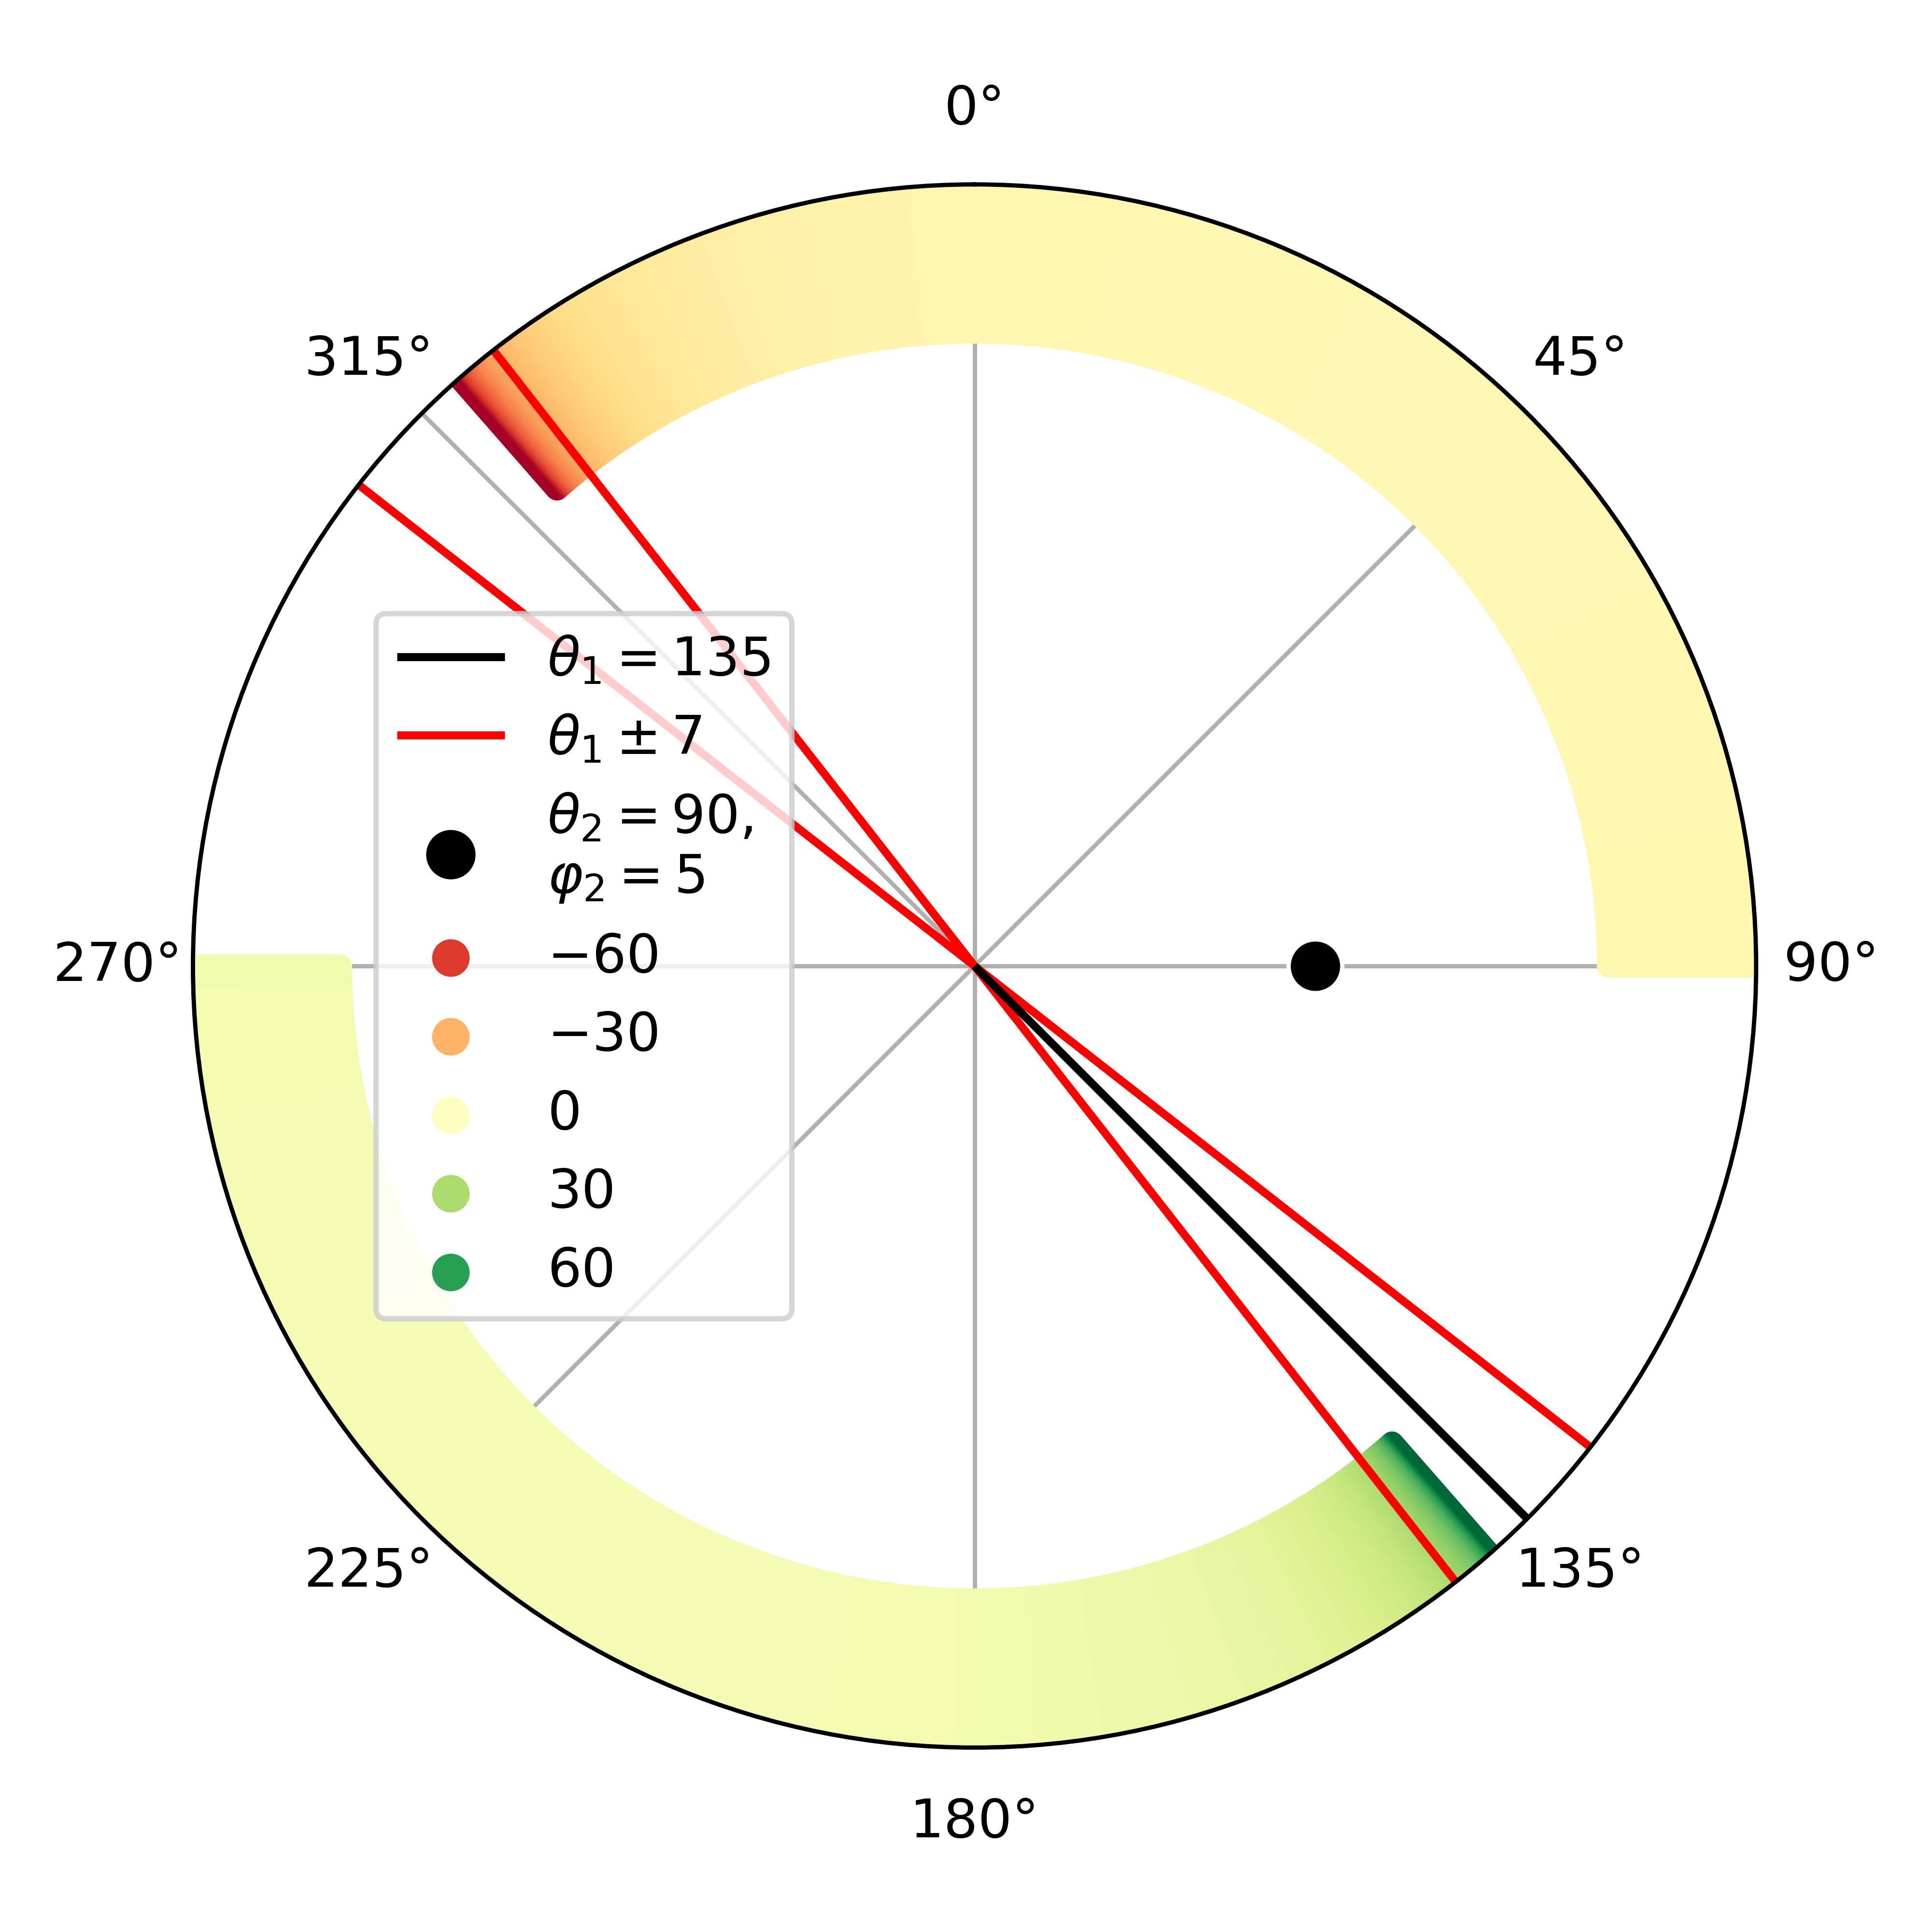
\includegraphics[width=\textwidth]{methods/tiltable-offset.pdf}%
    \caption[Sample Criteria: Tiltable \& Offset]{Two boolean criteria---tiltable and offset---used to assess how well a particular center describes a particular sample. For this sample, tiltable centers are those with a colorful rim (not the blank regions), where a tilt calculation can occur. Offset centers are those which are not within \ang{7} of colinear with the flow orientation; this region is bounded with red lines. Note that only direction-to-center matters for these criteria (not distance-to-center), since direction imposes the particular tilt axis (Figure~\ref{fig:fig:tilt-example}). Note that center-sample pair can be tiltable, offset, both, or neither, all of which are illustrated here.}
    \label{fig:tiltable-offset}
\end{figure}

A sample is well explained by a center if it is both tiltable and offset. Thus, an array of mapped samples is well explained by a center if a high fraction of those samples are both tiltable and offset. Thus, the score which captures how well each centers explains a particular set of discordant samples is the fraction of those samples which are both tiltable and offset.

\subsubsection{Goodness of Analytical Fit}\label{sec:inflation-center}

Instead, I need to consider a larger population of tilt-distance data points together. This increases the likelihood of recognizing a tilt pattern consistent with reservoir pressure change, i.e., a shape similar to those shown in Figures~\ref{fig:grav-topo-test},~\ref{fig:mogi-test}, and~\ref{fig:mogi-test-shallow-oblate}.

Finally, I perform a least-squares regression\footnote{Implemented using the \hltt{curve\_fit} function from the \hltt{scipy.optimize} Python module \parencite{2020SciPy-NMeth}} to fit an analytical tilt solution (Equation~\ref{eq:mogi-tilt}) to the valid sample subset (tiltable \& offset). Just as a linear regression computes the best-fitting slope and intercept, this process computes the best-fitting depth and energy parameters. In both cases, the best fit minimizes the mean square error:
\begin{equation}
    \frac{1}{n}\sum_{i}^{n}{\left[\acs{tilt}_i-\hat{\acs{tilt}}_i\right]}^2\label{eq:mse}
\end{equation}
for $n$ observations of the form $(\acs{dist}, \acs{tilt})$ where $\hat{\acs{tilt}}$ is evaluated at $\acs{dist}$ using the best-fit parameters. The details of the curve-fitting algorithm (Levenberg-Marquardt) are beyond the scope of this thesis, but one important difference from a simpler linear regression model is that the curve does not necessarily converge (successfully estimate a set of best-fitting parameters) for particularly messy datasets. Whether convergence occurs (and even the final parameter estimates) depends on initial parameter estimates and maximum number of iterations allowed before ``giving up'' on convergence.

Initial parameter estimates for inflation energy $\acs{epv} = \qty{7e19}{\J}$ if the mean tilt in the dataset is positive and \qty{-7e19}{\J} if the mean is negative. The initial depth estimate is $d = \qty{20}{\km}$ in either case. 500 iterations are allowed before a dataset is deemed non-convergent, i.e., not explainable by an analytical tilt model in the form of Equation~\eqref{eq:mogi-tilt}.

After performing each regression, I first assess the mathematical goodness of fit for each center's fitted tilt solution. First, I determine what fraction of the samples are. Recall that the regression only proceeds using this subset, so the fraction of the dataset involved provides important context for the second criterion: what is the \ac{RMSE} of the regression, if one converges at all? This statistic is the square root of Equation~\eqref{eq:mse}:
\begin{equation}
    \sqrt{\frac{1}{n}\sum_{i}^{n}{\left[\acs{tilt}_i-\hat{\acs{tilt}}_i\right]}^2}.\label{eq:rmse}
\end{equation}
It has the same units as \acs{tilt} (degrees) and provides a relative comparison of goodness-of-fit for regression results; smaller values indicate better fit. Taken together, the tiltable fraction and \ac{RMSE} associated with each center reflect the mathematical goodness-of-fit for each center candidate.

I use these fitted values and crucially, their associated error terms, to determine the likelihood that surface tilt actually occurred in the direction radial to the given center candidate. This approach is supported by Figure~\ref{fig:mogi-test-shallow-oblate}, which illustrates that even tilt resulting from shallow, oblate reservoirs within a topographic edifice can be fit well to the analytical Mogi tilt function. At this stage, I pay closer attention to the parameter error estimates (similar to an $R^2$ value for a linear regression) to determine whether \emph{any} axisymmetric tilt is likely to have occurred from this center, rather than the estimates themselves---although I treat any unrealistic parameter estimates with caution regardless of their goodness of fit.

This sequence of calculations is much more computationally expensive than the previous one, and a single realistic reservoir pressure change is unlikely to explain the entire dataset anyway. Therefore, I select smaller sample populations for this criterion, paying particular attention to the highly discordant flows near the southern summit region shown in Figure~\ref{fig:uphill-flows}.

\subsection{Depth, Radius, Aspect Ratio, \& Pressure Change}

After narrowing down the set of plausible inflation center locations (map view) in Section~\ref{sec:evaluation}, I use numerical model results to refine estimates for reservoir size, depth, shape, and pressure change.

Section~\ref{sec:evaluation} narrows down the plausible horizontal position of the reservoir center, but it can only play a limited role in identifying volcanologically plausible configurations.

Figure~\ref{fig:mogi-test-shallow-oblate} illustrates a key preliminary finding: map data which are well explained by an analytical Mogi tilt solutions are also likely to fit one or numerical results which approximate the deep, point-like reservoir assumed by \textcite{mogi_relations_1958}. Disagreement between numerical and analytical increases with the degree of analytical assumption violations.

The magmatic system below the summit of Olympus Mons is likely shallow and oblate. 

I use the same iterative optimization method (minimizing \acs{RMSE}) described in Section~\ref{sec:inflation-center}. In the absence of an explicit tilt equation parameterized by reservoir size, depth, shape, and pressure change, I perform a brute-force search through an array of numerical solutions at each iteration.

For each dataset (corresponding to a center candidate of interest) this process begins with a very coarse set of numerical model parameters. I use the \hlss{Parametric Sweep} tool in COMSOL to define a list of values to test for each parameter; the software produces and exports a displacement solution for each one. After